\section{RQ1: Where Does Network Awareness Pay?}
\label{sec:rq1}

\subsection{The link term must model the link \emph{queue}, not just its width}
Our first observation is that ``network-aware'' is not one policy. Table~\ref{tab:rq1main}
compares two network-aware scores against the network-blind reference LeastLoad on the
\emph{same} cells: $v_1$ adds only the transfer time $t^{\text{in}}+t^{\text{out}}$
(Eq.~\ref{eq:na1}), while $v_2$ additionally adds the link-queue drain time
(Eq.~\ref{eq:na2}). On the heterogeneous static network the difference is qualitative: for
\emph{data-heavy} traffic $v_1$ is \emph{harmful} ($+12.4\%$, worse in $5/5$ seeds) whereas
$v_2$ is strongly beneficial ($-66.7\%$, better in $5/5$). The reason is mechanical: the widest
link is attached to the slowest-computing worker, so a score that only knows ``this link is wide''
keeps sending traffic to a worker that is already behind, whereas a score that knows ``this link
is wide \emph{and currently drained by others}'' does not. Throughout the rest of the paper
``network awareness'' therefore means $v_2$ unless stated otherwise, and the $v_1$ row remains in
the tables because it is the convenient-but-wrong baseline that a practitioner may reach for.

\begin{table}[t]
\centering
\caption{Benefit boundary on the synthetic source (5 seeds, 20000 requests/cell,
$\rho=0.6$). Values are $\Delta$p95 relative to LeastLoad (\%, negative is better);
``stale'' is queue age 2 s / link age 30 s. $v_1$ = transfer-time-only
score, $v_2$ = transfer time $+$ link-queue drain. ``normal'' is a uniform-link control: a
network term can carry no information there, and it indeed delivers $\approx0$.}
\label{tab:rq1main}
\small
\begin{tabular}{@{}llrrrr@{}}
\toprule
& & \multicolumn{2}{c}{fresh} & \multicolumn{2}{c}{stale (2\,s / 30\,s)} \\
\cmidrule(lr){3-4}\cmidrule(lr){5-6}
Workload & Network & $v_1$ & $v_2$ & $v_1$ & $v_2$ \\
\midrule
compute-heavy & normal   & $0.0$   & $0.1$   & $0.0$   & $-0.5$ \\
compute-heavy & degraded & $-55.1$ & $-74.2$ & $-4.6$  & $-41.9$ \\
compute-heavy & unstable & $-9.8$  & $-11.1$ & $+3.1$  & $+5.1$ \\
data-heavy    & normal   & $0.0$   & $-0.3$  & $0.0$   & $-0.8$ \\
data-heavy    & degraded & $\mathbf{+12.4}$ & $\mathbf{-66.7}$ & $+0.2$ & $-70.9$ \\
data-heavy    & unstable & $+2.9$  & $-25.5$ & $+0.4$  & $-17.3$ \\
low-latency   & normal   & $0.0$   & $+0.4$  & $0.0$   & $-0.3$ \\
low-latency   & degraded & $-6.3$  & $-70.1$ & $-1.3$  & $-14.4$ \\
low-latency   & unstable & $+16.5$ & $-11.5$ & $+30.1$ & $+23.5$ \\
mixed         & normal   & $0.0$   & $-0.5$  & $0.0$   & $+0.7$ \\
mixed         & degraded & $-11.4$ & $-71.5$ & $-9.5$  & $-66.8$ \\
mixed         & unstable & $-3.1$  & $-26.2$ & $-4.3$  & $-8.9$ \\
\bottomrule
\end{tabular}
\end{table}

Three boundary conditions are visible already. First, the \emph{heterogeneous static} network
(\texttt{degraded}) is where network awareness earns its keep: $-67$ to $-74\%$ across workloads
and sources (Azure: $-77.1\%$/$-77.0\%$ for data-heavy/mixed; BurstGPT: $-66.9\%$/$-57.6\%$).
Second, on the \emph{volatile} network the benefit shrinks by roughly a factor of three
(synthetic $-17$ to $-26\%$, Azure $-37$ to $-40\%$), and on the burstiest source it can vanish
or invert (BurstGPT data-heavy/unstable: $+6.2\%$ mean, $+9.0\%$ median, better in only $2/5$
seeds). Third, the uniform-link control confirms the mechanism rather than merely being a
sanity check: with identical links everywhere there is nothing for the network term to
exploit, and the effect is $0.0\%$ for $v_1$ in $12/12$ cells.

\subsection{Network share is an on/off gate, not a dial}
\begin{figure}[t]
\centering
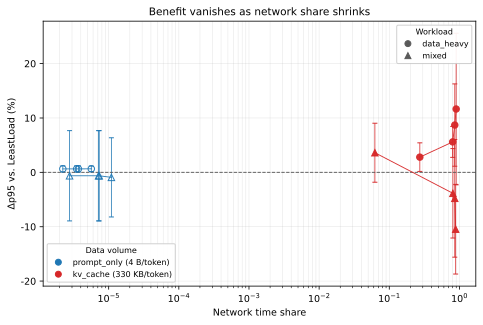
\includegraphics[width=\columnwidth]{figures/fig_benefit_vs_netshare.svg}
\caption{Benefit of the network-aware score against the network-blind baseline as a function of
the fraction of end-to-end time spent moving bytes. Each point is one configuration
(link-scale profile $\times$ workload class) at ten seeds; the two payload regimes are separated
by the vertical gap. Below a network share of a few percent the effect is indistinguishable from
zero.}
\label{fig:netshare}
\end{figure}
The cleanest boundary is the amount of traffic that crosses the network at all. Figure~\ref{fig:netshare} shows it across all four link-scale profiles. Holding
everything else fixed and switching the payload model from KV-cache transfer
(330 KB/token) to token-id-only (4 B/token) drives the measured network
share from $0.72$--$0.90$ to $0.00$--$0.02$, and the benefit from
$-54.2\%$/$-10.5\%$/$-5.4\%$ (compute-heavy/mixed/low-latency, heterogeneous static network) to
$-1.1\%$/$-0.6\%$/$-0.0\%$. Averaging over four link-scale profiles, the token-id-only regime
yields $\Delta$p95 of $-0.6$ to $+0.7\%$ for every workload --- indistinguishable from zero.
Note this is not a tautology of our network-share gate of \S\ref{sec:policy:adaptive}: the gate
only zeroes \emph{some} decisions (\texttt{w\_gated\_frac} $=0.09$--$0.19$ in the KV regime), and
the residual decisions still have to be scored correctly, which is why the KV regime retains a
$10$--$54\%$ effect rather than disappearing.

\subsection{Alignment: an important explanatory factor for the magnitude}
\label{sec:rq1:alignment}
We now vary \emph{only the pairing} between compute capacity and link bandwidth, holding both
multisets fixed, and re-run the full grid with ten seeds per cell. The result
(Table~\ref{tab:alignment}) is the paper's most robust mechanism finding: when the two rankings
agree ($\rho=+1$), network awareness yields $-3.3\%$ --- statistically distinguishable from zero
but operationally nothing --- while when they maximally disagree ($\rho=-1$) it yields
$-68.2\%$. Group tests over seeds separate the two regimes completely
(Cliff's $\delta=1.00$, Mann--Whitney $p=1.8\times10^{-4}$ for data-heavy/degraded; $\delta\ge
0.94$ and $p\le 4.4\times10^{-4}$ in all four workload$\times$network combinations), and the
pooled trend over the continuous alignment variable is $\rho_s=+0.72$
($p=2.6\times10^{-20}$, $n=120$): the better aligned the configuration, the smaller the benefit. Figure~\ref{fig:alignbars} shows the three alignment configurations side by side.

\begin{table}[t]
\centering
\caption{Alignment sweep (synthetic, 10 seeds, 12000 requests/cell; NetworkAware2 vs
LeastLoad). $\rho$ is the Spearman rank correlation between per-worker compute rate and
bandwidth (Eq.~\ref{eq:alignment}), measured on the configuration itself. ``aligned'' is a
control: the network term should add nothing, and does not.}
\label{tab:alignment}
\small
\begin{tabular}{@{}llrrrr@{}}
\toprule
Workload & Network & $\rho$ & $\Delta$p95 (\%) & 95\% CI & $n$ \\
\midrule
\multirow{3}{*}{data-heavy} & \multirow{3}{*}{degraded}
  & $-1.00$ & $-68.2$ & $\pm1.1$ & 10 \\
  & & $+0.50$ & $-30.0$ & $\pm1.3$ & 10 \\
  & & $+1.00$ & $-3.3$ & $\pm2.4$ & 10 \\
\multirow{3}{*}{data-heavy} & \multirow{3}{*}{unstable}
  & $-1.00$ & $-27.0$ & $\pm3.9$ & 10 \\
  & & $+0.50$ & $-26.1$ & $\pm7.3$ & 10 \\
  & & $+1.00$ & $-9.5$ & $\pm2.6$ & 10 \\
\multirow{3}{*}{mixed} & \multirow{3}{*}{degraded}
  & $-1.00$ & $-70.3$ & $\pm1.2$ & 10 \\
  & & $+0.50$ & $-35.4$ & $\pm3.0$ & 10 \\
  & & $+1.00$ & $-22.0$ & $\pm2.8$ & 10 \\
\multirow{3}{*}{mixed} & \multirow{3}{*}{unstable}
  & $-1.00$ & $-26.3$ & $\pm5.2$ & 10 \\
  & & $+0.50$ & $-29.7$ & $\pm7.6$ & 10 \\
  & & $+1.00$ & $-11.7$ & $\pm3.1$ & 10 \\
\bottomrule
\end{tabular}
\end{table}

\subsection{Comparison against standard and mechanism-level baselines}
\label{sec:rq1:baselines}
A reviewer's first question about a result like ours is whether the network-aware family is simply
beating weak baselines. We therefore add four comparison arms chosen so that each answers a
distinct question, all evaluated in the same cells with per-request pairing
(Table~\ref{tab:baselines}).

\textbf{(i) Is the baseline weak?} We compare against power-of-two-choices (P2C), the standard
strong baseline of the load-balancing literature and a fixture of LLM-serving evaluations. In our
setting P2C is \emph{not} a strong baseline: it beats LeastLoad in only $4/8$, $5/8$ and $3/8$
cells on the synthetic, Azure and BurstGPT sources respectively, and on Azure it is worse than
LeastLoad by up to $+17.2\%$. The reason is structural: with three workers in an anti-aligned
configuration, the lower-backlog of two randomly sampled workers is frequently the worker with
the slowest link. Every network-aware arm in this paper beats P2C in at least $6/8$ cells.
Our claim therefore does not rest on weak baselines --- but it also shows that a
\emph{network-blind} two-choice rule is a poor fit for heterogeneous links, which is worth stating
explicitly.

\textbf{(ii) How much does a global view buy?} \textsc{P2CNet} is the same score as
NetworkAware2 but evaluated on two randomly sampled workers instead of all of them. Across the 24
cells of three sources it wins 13 and loses 11 --- a coin flip --- and on the trace batches it is
sometimes substantially better (Azure, mixed/degraded/stale: $-63.3\%$ versus NetworkAware2's
$-40.5\%$). \emph{The network term is what matters; seeing every worker is not.} This has a
practical consequence: a network-aware router can be implemented with two probes per request
rather than $N$.

\textbf{(iii) Is the static bandwidth term redundant?} \textsc{CongestionOnly} is the
Aegis-style reduction of our score to its congestion term alone ($\text{backlog} +
\text{link drain}$), omitting the transfer-time term. It matches NetworkAware2 on the synthetic
source (and beats it in $4/8$ cells there, e.g.\ data-heavy/degraded/fresh: $-74.4\%$ versus
$-68.2\%$), but on both traces it is materially worse, especially once state is stale (Azure,
mixed/degraded/stale: $-27.9\%$ versus $-40.5\%$; data-heavy/degraded/stale: $-31.5\%$ versus
$-41.1\%$). The bandwidth term is therefore not redundant; a congestion-only score is sufficient
only when the links' widths are already known to the router.

\textbf{(iv) Max or sum?} \textsc{Bottleneck} replaces the sum of compute and network time with
their maximum, which is the resource-bottleneck view a max-flow placement takes. On the synthetic
source the sum wins in $8/8$ cells; on both traces the two are indistinguishable ($4/8$ each).
We read this as: at three workers with an anti-aligned configuration, the two resources are
\emph{substitutable} enough that summing is at least as good, and it is simpler.

\begin{table}[t]
\centering
\caption{Baselines vs.\ the network-blind reference (10 seeds, $\Delta$p95 vs.\ LeastLoad, \%,
negative is better). ``P2C'' = power-of-two-choices on backlog; ``P2CNet'' = two-choice on the
network-aware score; ``Cong.\ only'' = congestion term alone (Aegis-style); ``Bottleneck'' =
$\max(\text{compute},\text{network})$ (Helix-style). ``NA2'' = NetworkAware2.}
\label{tab:baselines}
\small
\setlength{\tabcolsep}{6pt}
\begin{tabular}{@{}llrrrrr@{}}
\toprule
Source & Cell & P2C & P2CNet & Cong.\ only & Bottleneck & NA2 \\
\midrule
Synthetic & d-heavy/degr./fresh & $+5.6$ & $-69.8$ & $\mathbf{-74.4}$ & $-66.4$ & $-68.2$ \\
Synthetic & mixed/unst./stale  & $-14.4$ & $-24.2$ & $-11.5$ & $-6.9$ & $-8.0$ \\
Azure & d-heavy/degr./fresh & $+17.2$ & $-76.2$ & $-76.4$ & $\mathbf{-77.8}$ & $-76.7$ \\
Azure & mixed/degr./stale  & $-6.5$ & $\mathbf{-63.3}$ & $-27.9$ & $-43.5$ & $-40.5$ \\
Azure & d-heavy/unst./stale & $-25.8$ & $-27.9$ & $-0.3$ & $+0.8$ & $-2.0$ \\
BurstGPT & mixed/degr./stale & $-15.9$ & $\mathbf{-50.1}$ & $-30.2$ & $-34.2$ & $-40.8$ \\
BurstGPT & mixed/unst./stale & $-23.3$ & $-20.1$ & $+2.1$ & $+1.2$ & $+7.2$ \\
\midrule
\multicolumn{2}{l}{cells beating LeastLoad (max.\ 8)} & $3$--$5$ & $7$--$8$ & $6$--$8$ & $6$--$8$ & $6$--$8$ \\
\bottomrule
\end{tabular}
\end{table}

\begin{figure}[t]
\centering
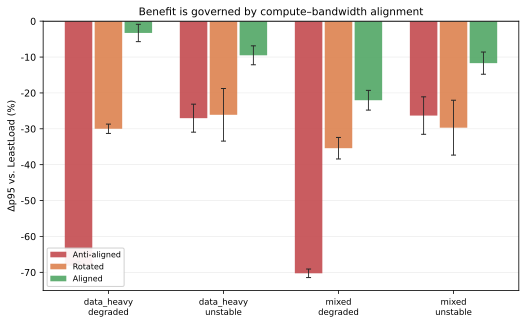
\includegraphics[width=\columnwidth]{figures/fig_alignment_bars.svg}
\caption{Benefit against the network-blind baseline for the three alignment configurations, four
workload$\times$network combinations, ten seeds each. Error bars are $95\%$ confidence intervals
over seeds. The aligned control sits at the origin; the anti-aligned configuration carries the
effect.}
\label{fig:alignbars}
\end{figure}
\begin{figure}[t]
\centering
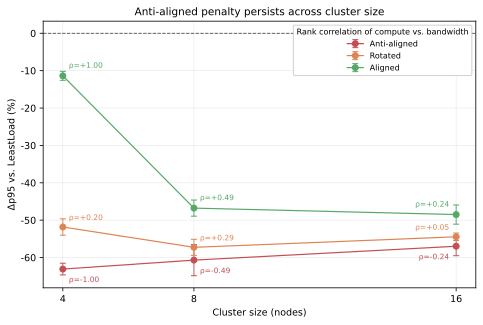
\includegraphics[width=\columnwidth]{figures/fig_alignment_vs_scale.svg}
\caption{The anti-aligned penalty as a function of cluster size, with the rank correlation
$\rho$ annotated at each point. The penalty is flat; what shrinks with size is the attainable
contrast (the $\rho$ values themselves).}
\label{fig:alignscale}
\end{figure}
\subsection{Does the effect survive scale, and is it real?}
Two natural objections follow. First, is the alignment effect an artifact of a three-worker
configuration? We re-run at 4, 8 and 16 workers. The anti-aligned penalty is essentially
\emph{flat} with size: $-63.1\%$, $-60.7\%$, $-57.0\%$ (all $p\le1.7\times10^{-3}$, Cliff
$\delta\ge0.84$). What \emph{does} shrink is the attainable contrast: with a compute ladder of
period four and an $N$-step bandwidth ramp, the extreme correlations become unreachable
($|\rho|$: $1.00$ at $N{=}3,4$; $0.49$ at $N{=}8$; $0.24$ at $N{=}16$). Within each size the
trend is still monotone and significant ($\rho_s=+0.94,+0.82,+0.78$). Reporting
``the effect decays with scale'' would therefore be wrong: the deployed (anti) benefit is
scale-robust, and what decays is our ability to construct a well-aligned \emph{control} at large
$N$ --- a manipulation limitation we disclose rather than a mechanism.

Second, could the benefit simply be LeastLoad ``getting lucky'' with links at larger sizes? We
probe this directly by recording, for every routed request, the bandwidth \emph{rank} of the
worker chosen (rank $1$ = widest link). Under the deployed anti-aligned configuration, LeastLoad
lands at ranks $2.08$, $2.88$, $4.57$, $7.93$ at $N=3,4,8,16$ against random-choice values of
$2.0$, $2.5$, $4.5$, $8.5$ --- i.e.~at or worse than random, never luckier (mean deviation
$0.28$ ranks over the whole range). Under the \emph{aligned} configuration it does land on good
links ($1.44$, $1.61$, $3.37$, $6.59$), and increasingly so with size, which is exactly why the
control benefit grows there. Figure~\ref{fig:alignscale} plots the penalty against cluster size, with the attained $\rho$ annotated at each point. The two configurations therefore differ in what a network-blind
router can achieve, not in whether that router is ``lucky''.

A third objection --- that our results are an artifact of the evaluator's own choices --- we
address in \S\ref{sec:threats}: the SLO definition, the two data-volume regimes, and the fact
that all four engineering coefficients are declared estimates. On load intensity we report a
caveat rather than a curve: the intensity sweep was run with the weaker $v_1$ score, and across
target intensities $0.30$--$0.90$ its effect on p95 ranges from $-15.6\%$ to $+30.8\%$
(mean per intensity level: $-3.0,+6.3,+0.3,-1.9,-2.7\%$, i.e.~no stable sign at all). The
$v_2$ results in this paper are all measured at $\rho=0.6$; extending the \emph{$v_2$} boundary
along the intensity axis is left as future work, and we flag it as the single largest gap in our
coverage.
